\begin{table*}[t]
\caption{Designed Duty Cycles for System}
\label{duty_cycle}
\begin{center}
\begin{tabular}{|c||c||c| |c| |c|}
\hline
Time Used & Output Torque (Nm) & Output Speed (RPM) & Actuator Torque (Nm) & Actuator Speed (RPM)\\
\hline
5\% & 2440 & 6.8 & 554.7 & 33.9\\
\hline
20\% & 1627 & 6.8 & 369.8 & 33.9\\
\hline
60\% & 542 & 15.3 & 123.3 & 76.3\\
\hline
15\% & 135 & 15.3 & 30.8 & 76.3\\
\hline
\end{tabular}
\end{center}
\end{table*}

In 2007 and 2008, NASA developed a manned rover prototype for planetary surfaces for future missions \cite{rover}.
This robotic vehicle is made up of six independent wheel modules, each with their own propulsion, steering, and both active and passive suspension.
In 2014, a new prototype wheel module was designed and created to analyze potential technologies that could be used in these applications.
In the new design layout, it was possible for the propulsion wheels to counter-rotate against the steering and put large shock loads into the steering system.
These requirements for a high load, compact package, high shock load, and tolerance of backlash lent themselves to the selection of a cycloidal drive for the steering actuator.
The prototype wheel module layout can be seen in Fig \ref{wheel_module}.

\begin{figure}[t]
   \centering
   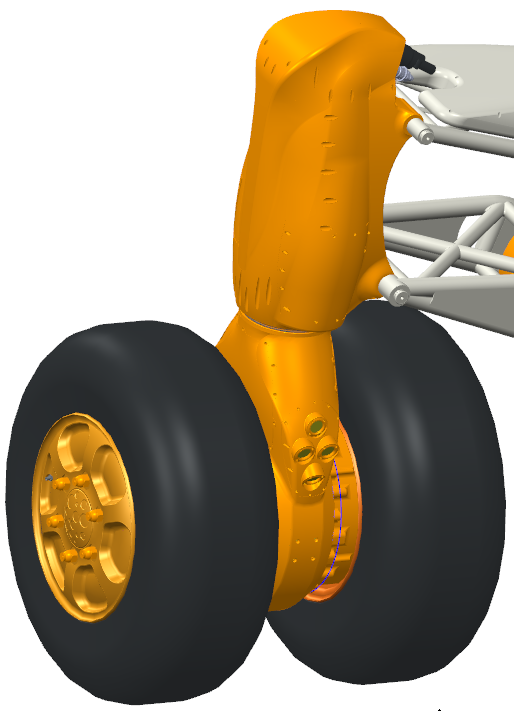
\includegraphics[width=0.50\linewidth]{images/wheel_module_CAD}
   \caption{CAD model of rover wheel module prototype.
   Suspension arms hold the steering column.
   Each wheel has an in-wheel propulsion motor.}
   \label{wheel_module}
\end{figure}

Based on the load cases, the actuator was required to output a stall torque of 2,440 Nm (1800 ft-lb) with a max output speed of 1.57 rad/s (90 deg/s) at 1,626 Nm (1200 ft-lb).
The required torque/speed data points are presented in Table \ref{duty_cycle} with an assumed loss of 88\% chosen based on the available literature.
The actuator layout for the vehicle placed the motor and cycloid off center of the steering axis with an additional 5:1 reduction into the steering column, thus decreasing the torque needed for the cycloid output, but increasing the potential shock loading.


Many sources have laid out the design parameters for these drives and the equations are provided below for completeness.
Shin and Kwon \cite{on_the_lobe} presented the mathematical definition of the cycloid profile as

\begin{equation} \label{eq:1}
C_x = R cos\phi -R_r cos(\phi + \psi) - e cos((Z_1 + 1)\phi) 
\end{equation}
\begin{equation} \label{eq:2}
C_y = -R sin\phi + R_r sin(\phi + \psi) + e sin((Z_1 + 1)\phi) 
\end{equation}
\begin{equation} \label{eq:3}
\psi = tan^{-1} \lbrack\frac{sin(Z \phi)}{cos(Z \phi) - R / (e(Z + 1))}\rbrack 
\end{equation}

where \textphi\ is the angle of the input shaft and \textpsi\ is the angle of contact between the outer pin and the cycloid lobe.


Using both the formula for the reduction in diameter of the cycloid disk to account for machine tolerances \cite{machine_design} \cite{design_and_application} as well as Ye et al.'s formula for calculating the limit of undercutting \cite{ye}, the allowable sizes of the profiles and pins can be determined.
Sensinger \cite{unified_approach} laid out simple equations for calculating stress on the lobes and pins that has been further modelled and studied by others.
The force on the cam for calculating the bearing load with eccentricity e, ratio Z , and torque T is

\begin{equation} \label{eq:4}
F_{cam} = \frac{T}{e Z}.
\end{equation}

The simplified stress equations where \textit{R} and \textit{R\textsubscript{r}} are defined above, \textit{t} is the contact thickness, and \textit{b} is the width of contact determined by (\ref{eq:7}) and (\ref{eq:8}) are

\begin{equation} \label{eq:5}
F = \frac{T}{R - R_r}
\end{equation}
\begin{equation} \label{eq:6}
\sigma = \frac{2F}{\pi b t} (3 + 4v^2)
\end{equation}
\begin{equation} \label{eq:7}
b = \sqrt{\frac{4F (v-v_1^2) /E_1 + (1 - v_2^2)/E_2}{\pi l (1/R_1 + 1/R_2)}}
\end{equation}
\begin{equation} \label{eq:8}
R_2 = \frac{(R-eZ - e)^3}{R-e(Z-1)^2} - R_r.
\end{equation}

\begin{figure}[!b]
   \centering
   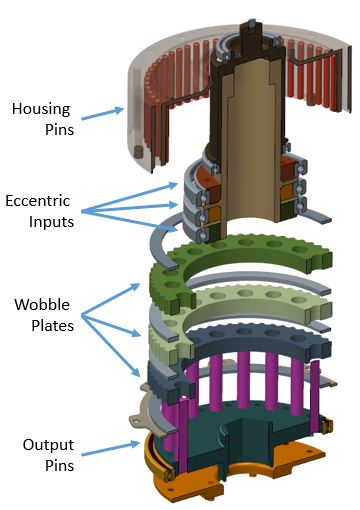
\includegraphics[width=0.75\linewidth]{images/exploded_labeled}
   \caption{Exploded view of the cycloidal reducer.
   Three wobble plates are driven by the input shaft with 120\textdegree\ offsets.
   The ring pins are are free pins inserted in the housing.
   The output has pins that run through all three wobble plates to harness the counter-rotation for the drive output.}
   \label{cycloid_exploded}
\end{figure}

The stress calculations and trading of overall size and ratio led to a necessary plate thickness of 3.81cm (1.5in) ( (TODO: Verify).
Instead of a single large plate however, three wobble plates were selected to split the load on the central input shaft across three bearings as well as to build in natural balance for the actuator.
If a single plate is used, a counterbalance must be added to avoid extreme vibration.
In this case, the three plates were offset 120\textdegree\ to balance these loads and vibration.
This adds additional stack height to the system to allow separation between the plates.
This arrangement allows the large design loads to be able to be handled by the system.
The exploded view of this design can be seen in Fig \ref{cycloid_exploded}.

The actuator uses a Parker Frameless Kit Motor, model K089200-7Y with no hall effect sensors and is commutated using a Renishaw RM-44 magnetic incremental and absolute position sensor.
The final reduction is 59:1 going before into the final 5:1 output gear.
The system is commutated using the delta hysteresis commutation scheme \cite{electric_machines} using velocity control.

